\documentclass[11pt,a4paper]{article}
\usepackage[margin=1in]{geometry}
\usepackage{graphicx}
\usepackage{tikz}
\usepackage{amsmath}
\usepackage{hyperref}
\usepackage{listings}
% Define additional languages for listings (SQL, bash) and JavaScript
\lstdefinelanguage{SQL}{
  morekeywords={SELECT,FROM,WHERE,GROUP,BY,ORDER,LIMIT,CREATE,TABLE,PARTITION,CLUSTER,OPTIONS,WITH,AS,WINDOW,OVER,ROWS,PRECEDING,CURRENT,DATE,INTERVAL,ARRAY,AGG,STRUCT,REPLACE,FUNCTION,RETURNS,LANGUAGE,REMOTE,CONNECTION,UPDATE,INSERT,DELETE,JOIN,LEFT,RIGHT,INNER,OUTER,HAVING,DISTINCT},
  sensitive=false,
  morecomment=[l]{--},
  morestring=[b]',
  morestring=[b]"
}
\lstdefinelanguage{bash}{
  morekeywords={sudo,apt,apt-get,yum,pacman,brew,systemctl,service,export,echo,cd,ls,cp,mv,rm,mkdir,tar,gzip,gunzip,cat,grep,find,ssh,scp,gcloud},
  sensitive=true,
  morecomment=[l]{\#},
  morestring=[b]",
  morestring=[b]'
}
\lstdefinelanguage{JavaScript}{
  keywords={break,case,catch,continue,debugger,default,delete,do,else,false,finally,for,function,if,in,instanceof,new,null,return,switch,this,throw,true,try,typeof,var,let,const,yield,async,await},
  morecomment=[l]{//},
  morecomment=[s]{/*}{*/},
  morestring=[b]",
  morestring=[b]'
}
\usepackage{xcolor}
\usepackage{booktabs}
\usepackage{enumitem}
\usepackage{float} % For forcing figure placement with [H]

\usetikzlibrary{shapes.geometric, arrows, positioning, fit, backgrounds}

% Define colors
\definecolor{codegreen}{rgb}{0,0.6,0}
\definecolor{codegray}{rgb}{0.5,0.5,0.5}
\definecolor{codepurple}{rgb}{0.58,0,0.82}
\definecolor{backcolour}{rgb}{0.95,0.95,0.92}

% Code listing style
\lstdefinestyle{mystyle}{
    backgroundcolor=\color{backcolour},   
    commentstyle=\color{codegreen},
    keywordstyle=\color{magenta},
    numberstyle=\tiny\color{codegray},
    stringstyle=\color{codepurple},
    basicstyle=\ttfamily\footnotesize,
    breakatwhitespace=false,         
    breaklines=true,                 
    captionpos=b,                    
    keepspaces=true,                 
    numbers=left,                    
    numbersep=5pt,                  
    showspaces=false,                
    showstringspaces=false,
    showtabs=false,                  
    tabsize=2
}
\lstset{style=mystyle}

\title{\textbf{Distributed Stock Price Prediction Using Mean Reversion Signals}\\
\large Refined Architecture Document}
\author{Cloud-Native Trading System}
\date{November 9, 2025}

\begin{document}

\maketitle

% \begin{abstract}
% This document presents a refined two-phase architecture for a mean reversion trading system built on Google Cloud Platform's serverless infrastructure. Phase 1 performs daily batch screening of equities using statistical tests (ADF, Hurst exponent, Variance Ratio) executed in BigQuery. Phase 2 monitors screened candidates in real-time, computes technical indicators, and emits trading signals via Pub/Sub. The architecture emphasizes cost efficiency, scalability, and operational simplicity while maintaining low latency for signal generation.
% \end{abstract}

% \tableofcontents
% \newpage

\section{System Overview}

\subsection{Design Principles}
\begin{itemize}[leftmargin=*]
    \item \textbf{Serverless-first}: Minimize operational overhead and cost by using managed services
    \item \textbf{Separation of concerns}: Batch analytics (Phase 1) decoupled from real-time monitoring (Phase 2)
    \item \textbf{Cost optimization}: Use Cloud Functions/Cloud Run instead of persistent VMs where possible
    \item \textbf{Scalability}: Leverage BigQuery's MPP architecture for parallel processing
    \item \textbf{Low latency}: Direct indicator computation without unnecessary data serialization
\end{itemize}

\subsection{Key Components}
\begin{enumerate}[leftmargin=*]
    \item \textbf{Cloud Scheduler}: Triggers daily batch screening workflow
    \item \textbf{Cloud Function/Run}: Serverless compute for data ingestion
  \item \textbf{BigQuery}: Analytical warehouse with UDFs (ADF, Hurst, Variance Ratio) -- ADF implemented as SQL UDF (approximate) rather than remote function
    \item \textbf{Firestore/Redis}: Low-latency watchlist storage
  \item \textbf{Cloud Run/VM}: Real-time monitoring service
  \item \textbf{Pub/Sub (Prices)}: Serverless bus for 1m/5m price bars (per-symbol ordering keys)
  \item \textbf{Pub/Sub (Signals)}: Event bus for downstream trading signals
    \item \textbf{Alpha Vantage/Polygon.io}: Real-time market data provider
\end{enumerate}

\section{Architecture Diagram}

\begin{figure}[H] % Force placement directly here
\centering
\begin{minipage}{\textwidth}
\centering
\resizebox{0.95\textwidth}{!}{%
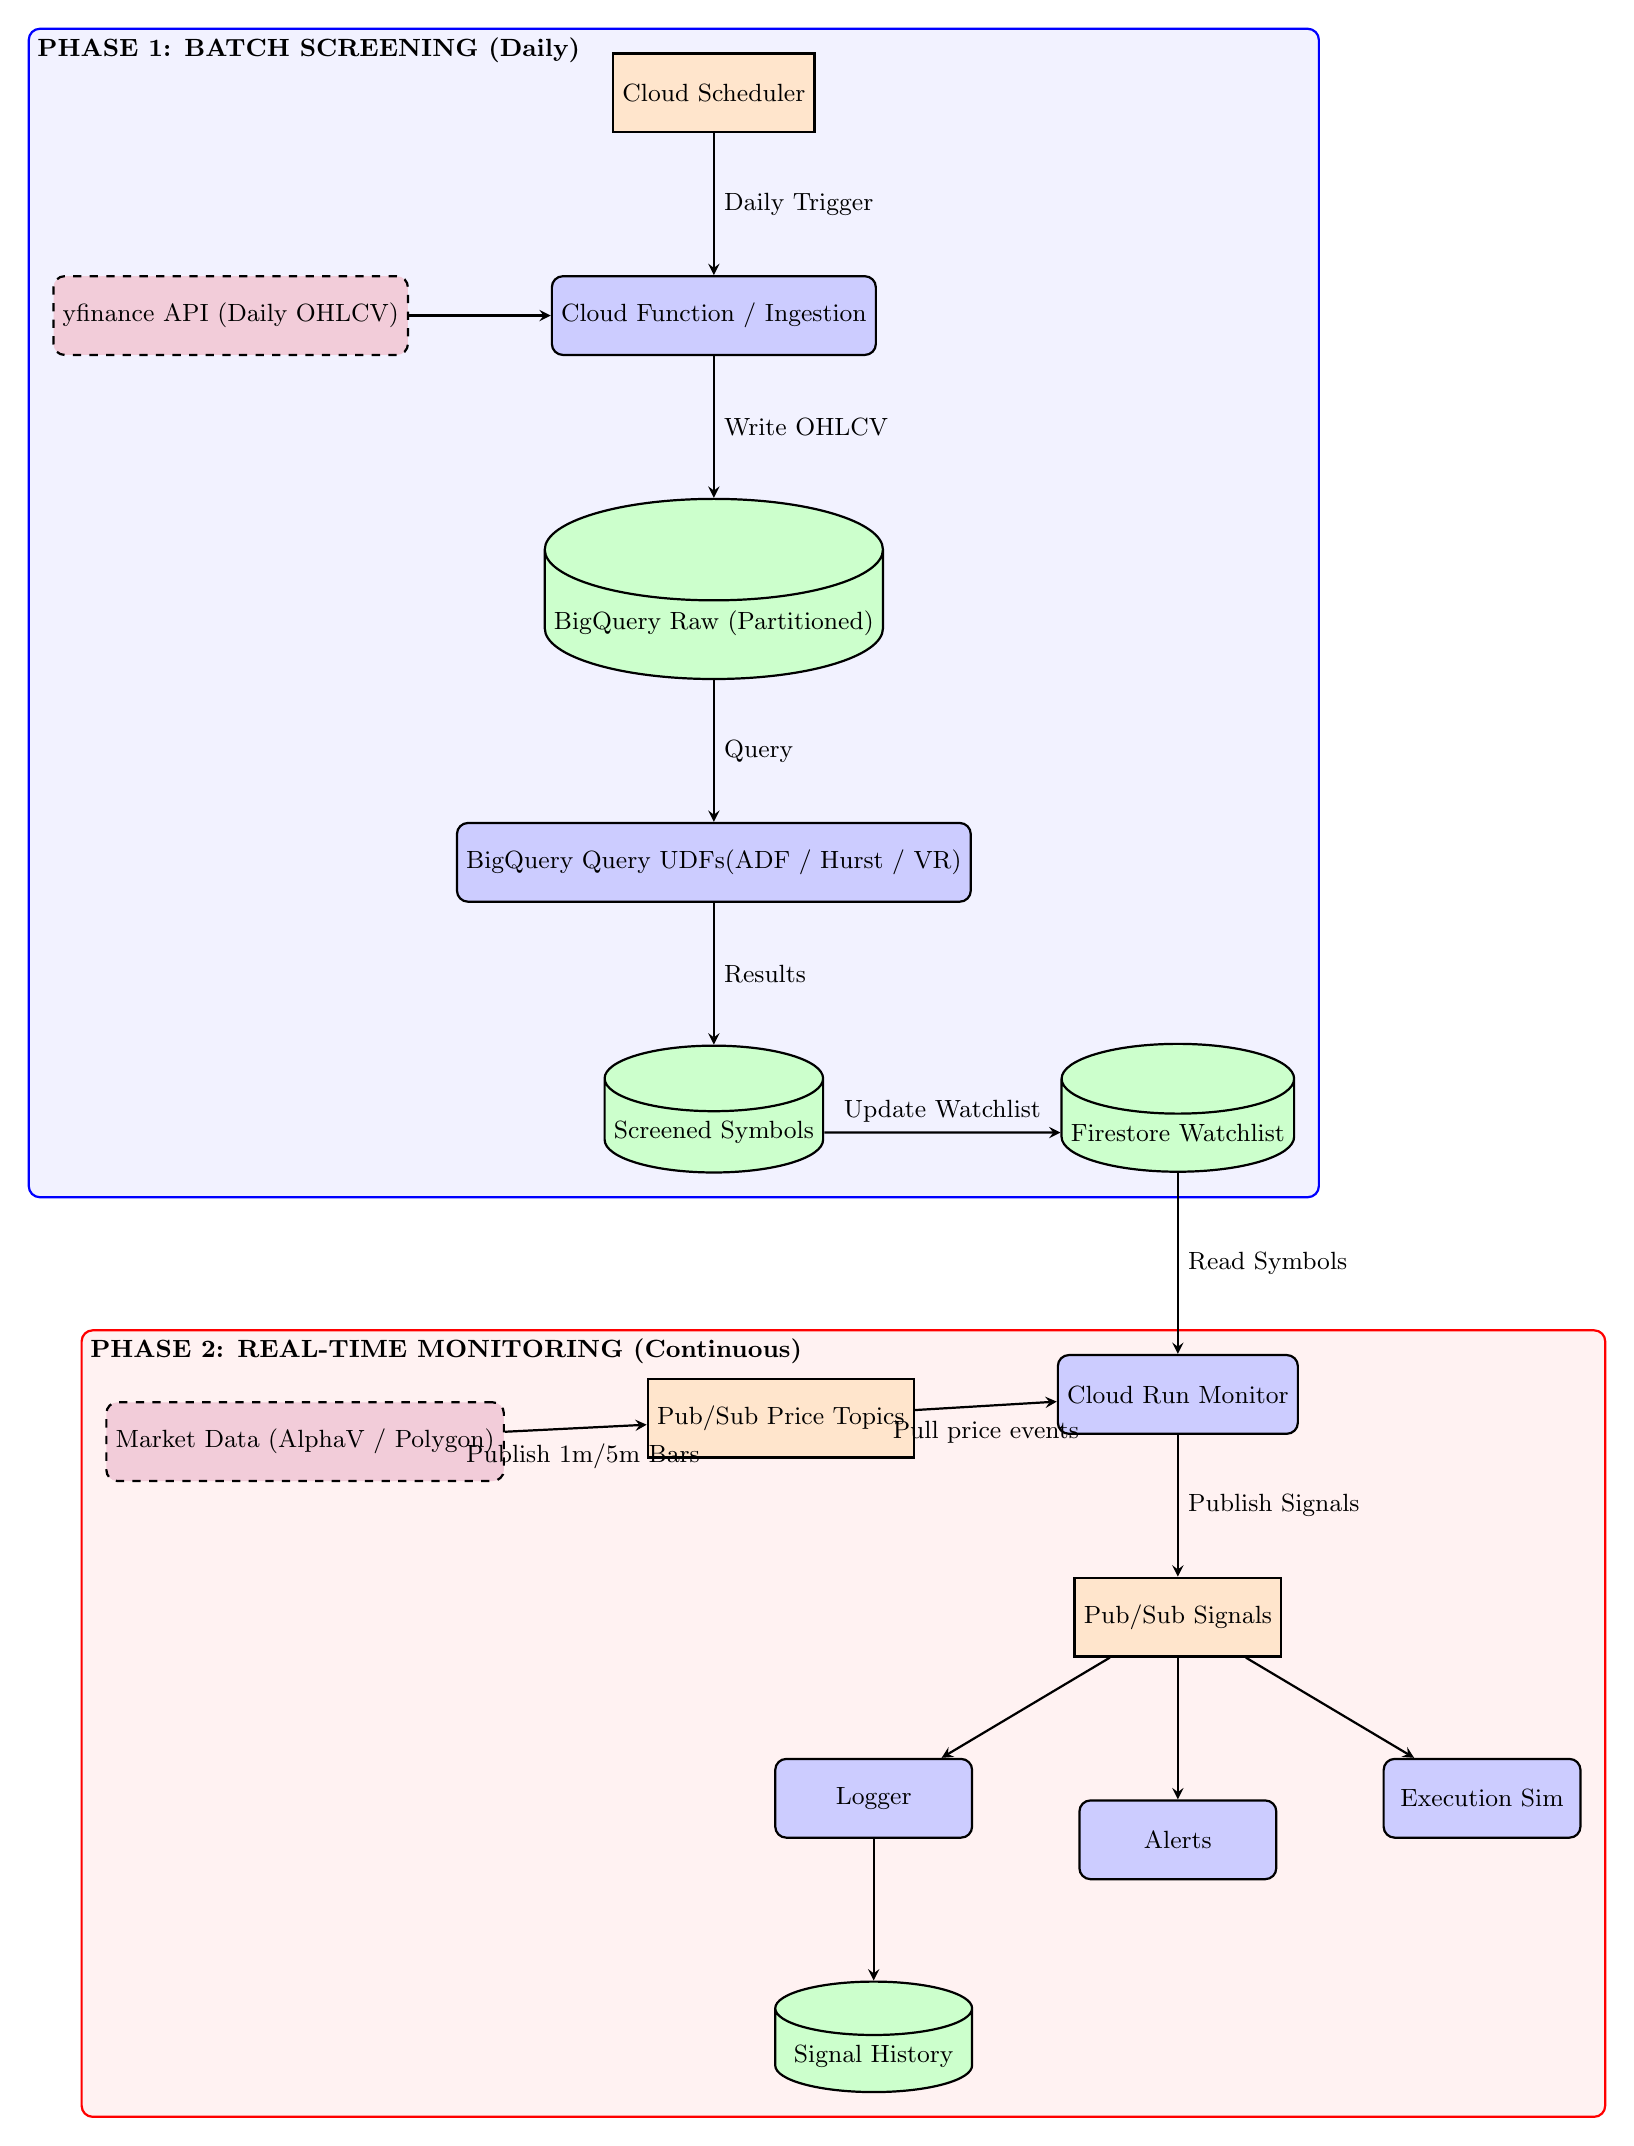
\begin{tikzpicture}[
  node distance=1.8cm,
    every node/.style={font=\small},
    process/.style={rectangle, rounded corners, minimum width=2.5cm, minimum height=1cm, text centered, draw=black, fill=blue!20, thick},
    storage/.style={cylinder, shape border rotate=90, aspect=0.3, minimum width=2.5cm, minimum height=1cm, text centered, draw=black, fill=green!20, thick},
    service/.style={rectangle, minimum width=2.5cm, minimum height=1cm, text centered, draw=black, fill=orange!20, thick},
    external/.style={rectangle, rounded corners, minimum width=2.5cm, minimum height=1cm, text centered, draw=black, fill=purple!20, thick, dashed},
    arrow/.style={thick,->,>=stealth}
]

% Phase 1: Batch Screening
\node (scheduler) [service] {Cloud Scheduler};
\node (function) [process, below=of scheduler] {Cloud Function / Ingestion};
\node (yfinance) [external, left=of function] {yfinance API (Daily OHLCV)};
\node (bq_raw) [storage, below=of function] {BigQuery Raw (Partitioned)};
\node (bq_query) [process, below=of bq_raw] {BigQuery Query UDFs\newline (ADF / Hurst / VR)};
\node (bq_screened) [storage, below=of bq_query] {Screened Symbols};
\node (firestore) [storage, right=3cm of bq_screened] {Firestore Watchlist};

% Phase 2: Real-time Monitoring with Pub/Sub
\node (monitor) [process, below=2.3cm of firestore] {Cloud Run Monitor};
\node (kafka) [service, left=of monitor, yshift=-0.3cm] {Pub/Sub Price Topics};
\node (market_data) [external, left=of kafka, yshift=-0.3cm] {Market Data (AlphaV / Polygon)};
\node (pubsub) [service, below=of monitor] {Pub/Sub Signals};
\node (subscriber1) [process, below left=of pubsub] {Logger};
\node (subscriber2) [process, below=of pubsub] {Alerts};
\node (subscriber3) [process, below right=of pubsub] {Execution Sim};
\node (bq_signals) [storage, below=of subscriber1] {Signal History};

% Arrows - Phase 1
\draw [arrow] (scheduler) -- (function) node[midway,right] {Daily Trigger};
\draw [arrow] (yfinance) -- (function);
\draw [arrow] (function) -- (bq_raw) node[midway,right] {Write OHLCV};
\draw [arrow] (bq_raw) -- (bq_query) node[midway,right] {Query};
\draw [arrow] (bq_query) -- (bq_screened) node[midway,right] {Results};
\draw [arrow] (bq_screened) -- (firestore) node[midway,above] {Update Watchlist};

% Arrows - Phase 2
\draw [arrow] (firestore) -- (monitor) node[midway,right] {Read Symbols};
\draw [arrow] (market_data) -- (kafka) node[pos=0.55,below,yshift=-2pt] {Publish 1m/5m Bars};
\draw [arrow] (kafka) -- (monitor) node[pos=0.5,below,yshift=-2pt] {Pull price events};
\draw [arrow] (monitor) -- (pubsub) node[midway,right] {Publish Signals};
\draw [arrow] (pubsub) -- (subscriber1);
\draw [arrow] (pubsub) -- (subscriber2);
\draw [arrow] (pubsub) -- (subscriber3);
\draw [arrow] (subscriber1) -- (bq_signals);

% Background boxes
\begin{scope}[on background layer]
    \node[draw=blue, thick, rounded corners, fit={(scheduler) (function) (yfinance) (bq_raw) (bq_query) (bq_screened) (firestore)}, fill=blue!5, inner sep=0.3cm, label={[anchor=north west]north west:\textbf{PHASE 1: BATCH SCREENING (Daily)}}] {};
    \node[draw=red, thick, rounded corners, fit={(monitor) (market_data) (pubsub) (subscriber1) (subscriber2) (subscriber3) (bq_signals)}, fill=red!5, inner sep=0.3cm, label={[anchor=north west]north west:\textbf{PHASE 2: REAL-TIME MONITORING (Continuous)}}] {};
\end{scope}

\end{tikzpicture}%
}% end resizebox
\end{minipage}
\caption{Two-Phase Cloud-Native Trading Architecture}
\label{fig:architecture}
\end{figure}

\newpage
\section{Phase 1: Batch Screening (Daily)}

\subsection{Workflow Description}
Phase 1 executes once daily to identify mean-reverting stocks from the entire universe. This phase prioritizes thoroughness and statistical rigor over speed.

\subsection{Step-by-Step Process}

\subsubsection{Step 1: Scheduled Trigger}
\textbf{Component}: Cloud Scheduler

\begin{itemize}[leftmargin=*]
    \item Triggers daily at market close (e.g., 4:30 PM ET)
    \item Invokes Cloud Function via HTTP POST
\end{itemize}

\subsubsection{Step 2: Data Ingestion}
\textbf{Component}: Cloud Function (Python 3.11)

\textbf{Responsibilities}:
\begin{itemize}[leftmargin=*]
    \item Fetch daily OHLCV data for entire universe (e.g., S\&P 500, Russell 3000)
    \item Use \texttt{yfinance} library with batch requests
    \item Write directly to BigQuery using streaming inserts or load jobs
    \item Handle retries and logging
\end{itemize}

\textbf{Why Cloud Function instead of VM?}
\begin{itemize}[leftmargin=*]
    \item No idle costs (only pay for execution time)
    \item Auto-scaling and fault tolerance built-in
    \item Typical execution: 2-5 minutes/day
\end{itemize}

\textbf{Alternative}: Cloud Run for longer execution times (up to 60 minutes vs. 9 minutes for Cloud Functions)

\subsubsection{Step 3: Statistical Analysis}
\textbf{Component}: BigQuery with User-Defined Functions (UDFs)

BigQuery executes a single analytical query that:
\begin{enumerate}[leftmargin=*]
    \item Computes rolling windows (20, 50, 200 days) using window functions
    \item Calculates mean reversion statistics via custom UDFs:
    \begin{itemize}
        \item \textbf{Augmented Dickey-Fuller (ADF) test}: Tests for unit root (stationarity)
        \item \textbf{Hurst exponent}: Measures mean reversion ($H < 0.5$) vs. trending ($H > 0.5$)
        \item \textbf{Variance Ratio (VR) test}: Detects deviations from random walk
    \end{itemize}
    \item Applies filters (liquidity, bid-ask spread, ADV constraints)
    \item Ranks candidates by composite score
\end{enumerate}

\textbf{UDF Implementation Options}:
\begin{itemize}[leftmargin=*]
    \item \textbf{Option A}: JavaScript UDF (runs in BigQuery, fastest but limited libraries)
  \item \textbf{Option B}: Python Remote Function (calls Cloud Function/Run) — not used in this project; we standardize on UDFs (including an approximate ADF UDF)
\end{itemize}

	extbf{Recommended}: Implement ADF, Hurst, and Variance Ratio as BigQuery UDFs. For ADF, use the provided approximate UDF for screening; reserve precise Python stats for offline backtesting if needed.

\subsubsection{Step 4: Results Storage}
\textbf{Components}: BigQuery (screened symbols table) + Firestore (watchlist)

\begin{itemize}[leftmargin=*]
    \item BigQuery table stores full screening results with metadata:
    \begin{itemize}
        \item Symbol, screening date, ADF p-value, Hurst exponent, VR statistic
        \item Computed thresholds (Bollinger Bands, z-score levels)
        \item Liquidity metrics (ADV, spread)
    \end{itemize}
    \item Firestore document stores lightweight watchlist for real-time service:
    \begin{itemize}
        \item Just symbols and trigger conditions
        \item Updated via Cloud Function trigger or direct BigQuery export
    \end{itemize}
\end{itemize}

\subsection{Data Schema}

\subsubsection{BigQuery Raw Data Table}
\begin{lstlisting}[language=SQL, caption=Raw OHLCV Schema (Partitioned by date)]
CREATE TABLE `project.dataset.ohlcv_daily`
(
  symbol STRING NOT NULL,
  date DATE NOT NULL,
  open FLOAT64,
  high FLOAT64,
  low FLOAT64,
  close FLOAT64,
  volume INT64,
  adj_close FLOAT64
)
PARTITION BY date
CLUSTER BY symbol
OPTIONS(
  partition_expiration_days=1095,  -- 3 years retention
  require_partition_filter=TRUE
);
\end{lstlisting}

\subsubsection{BigQuery Screened Symbols Table}
\begin{lstlisting}[language=SQL, caption=Screening Results Schema]
CREATE TABLE `project.dataset.screened_symbols`
(
  screening_date DATE NOT NULL,
  symbol STRING NOT NULL,
  adf_statistic FLOAT64,
  adf_pvalue FLOAT64,
  hurst_exponent FLOAT64,
  vr_statistic FLOAT64,
  mean_reversion_score FLOAT64,
  bb_upper FLOAT64,
  bb_lower FLOAT64,
  bb_period INT64,
  avg_volume FLOAT64,
  avg_spread FLOAT64
)
PARTITION BY screening_date
CLUSTER BY mean_reversion_score;
\end{lstlisting}

\subsubsection{Firestore Watchlist Document}
\begin{lstlisting}[language=Python, caption=Firestore Document Structure]
{
  "updated_at": "2025-11-09T16:30:00Z",
  "symbols": [
    {
      "symbol": "AAPL",
      "bb_lower": 148.50,
      "bb_upper": 152.30,
      "rsi_oversold": 30,
      "rsi_overbought": 70,
      "hurst": 0.42
    },
    // ... more symbols
  ]
}
\end{lstlisting}

\newpage
\section{Phase 2: Real-Time Monitoring (Continuous)}

\subsection{Workflow Description}
Phase 2 continuously monitors the screened watchlist, fetches intraday prices, computes technical indicators locally, and publishes trading signals when conditions are met.

\subsection{Step-by-Step Process}

\subsubsection{Step 1: Service Initialization}
\textbf{Component}: Cloud Run or Compute Engine VM

The monitoring service starts and:
\begin{enumerate}[leftmargin=*]
    \item Reads the watchlist from Firestore
    \item Establishes connection to market data provider
    \item Initializes indicator calculation state (e.g., MACD buffers)
    \item Subscribes to Pub/Sub for configuration updates (optional)
\end{enumerate}

\textbf{Cloud Run vs. VM Decision}:
\begin{itemize}[leftmargin=*]
    \item \textbf{Cloud Run}: Better for cost if market hours only (6.5 hrs/day)
    \item \textbf{VM (e2-micro)}: Better if running 24/7 or need persistent state
    \item \textbf{Recommendation}: Start with Cloud Run, migrate to VM if needed
\end{itemize}

\subsubsection{Step 2: Market Data Ingestion via Pub/Sub}
  	extbf{Data Source}: Alpha Vantage, Polygon.io, or IEX Cloud $\Rightarrow$ Pub/Sub Price Topics

\textbf{Why not yfinance for real-time?}
\begin{itemize}[leftmargin=*]
    \item yfinance is designed for historical data only
    \item Rate limits and unreliable for sub-hourly intervals
    \item No official API; scrapes Yahoo Finance (terms of service violations)
\end{itemize}

	extbf{Ingestion Pattern}
\begin{itemize}[leftmargin=*]
  \item \textbf{Producer}: Cloud Run service (or lightweight container) polls market data provider APIs and publishes normalized OHLCV bars to Pub/Sub topics (\texttt{prices-1m}, \texttt{prices-5m}) using ordering keys per symbol (e.g., \texttt{AAPL})
  \item \textbf{Topics}: Message ordering enabled; acknowledgement deadline tuned (e.g., 30s). Retention for unacknowledged messages max 7 days.
  \item \textbf{Consumer}: Monitoring service creates one subscription per interval or a single subscription with filtering; processes only watched symbols from Firestore
  \item \textbf{Backpressure}: Autoscaling Cloud Run instances + Pub/Sub flow control (max messages in-flight) ensure bounded memory; explicit acks after processing
\end{itemize}

\subsubsection{Step 3: Indicator Computation}
\textbf{Local Processing (No Pub/Sub Yet!)}

For each price update, compute:
\begin{itemize}[leftmargin=*]
    \item \textbf{MACD} (Moving Average Convergence Divergence): Trend momentum
    \item \textbf{RSI} (Relative Strength Index): Overbought/oversold
    \item \textbf{ADX} (Average Directional Index): Trend strength
    \item \textbf{Bollinger Bands}: Volatility and reversion bands
    \item \textbf{Z-score}: Current price vs. rolling mean
\end{itemize}

\textbf{Key Design Point}: Indicators are computed \textit{where data is fetched}. Do NOT publish raw prices to Pub/Sub and compute elsewhere—this adds latency and complexity.

\subsubsection{Step 4: Signal Logic}
Apply rules to generate trading signals:

\begin{lstlisting}[language=Python, caption=Example Signal Logic]
def check_buy_signal(symbol, price, indicators):
    """
    Buy signal for mean reversion entry
    """
    bb_lower = indicators['bb_lower']
    rsi = indicators['rsi']
    z_score = indicators['z_score']
    
    conditions = [
        price <= bb_lower,           # Below lower band
        rsi < 30,                    # Oversold
        z_score < -2.0,              # 2 std devs below mean
        indicators['adx'] < 25       # Weak trend (good for MR)
    ]
    
    if all(conditions):
        return {
            'action': 'BUY',
            'symbol': symbol,
            'price': price,
            'confidence': 0.85,
            'reason': 'Mean reversion setup'
        }
    return None
\end{lstlisting}

\subsubsection{Step 5: Signal Publication}
\textbf{Component}: Pub/Sub Topic

When a signal is generated:
\begin{enumerate}[leftmargin=*]
    \item Serialize signal to JSON
    \item Publish to \texttt{trading-signals} Pub/Sub topic
    \item Include timestamp, symbol, action, price, confidence, metadata
\end{enumerate}

\textbf{Message Schema}:
\begin{lstlisting}[language=Python, caption=Pub/Sub Signal Message]
{
  "timestamp": "2025-11-09T14:35:22.123Z",
  "symbol": "AAPL",
  "action": "BUY",
  "side": "LONG",
  "price": 148.75,
  "confidence": 0.85,
  "indicators": {
    "rsi": 28.5,
    "z_score": -2.15,
    "bb_lower": 148.50
  },
  "reason": "Mean reversion entry",
  "strategy": "bollinger_rsi_mr_v1"
}
\end{lstlisting}

\subsubsection{Step 6: Signal Consumption}
\textbf{Subscribers}: Multiple services consume signals from Pub/Sub

\begin{enumerate}[leftmargin=*]
    \item \textbf{Logger Service}: Writes all signals to BigQuery for backtesting and analysis
    \item \textbf{Alert Service}: Sends notifications (email, Slack, SMS) to traders
    \item \textbf{Execution Simulator}: Paper trading service that simulates order fills
    \item \textbf{Risk Monitor}: Checks position limits, exposure constraints
    \item \textbf{Dashboard}: Real-time web UI showing active signals
\end{enumerate}

\subsection{Implementation Details}

\subsubsection{Monitoring Service Structure}
\begin{lstlisting}[language=Python, caption=Real-Time Monitoring Service (Pub/Sub Subscriber)]
import json
import time
from collections import deque, defaultdict
from google.cloud import firestore, pubsub_v1
import pandas as pd
import ta  # Technical Analysis library

PRICE_WINDOW = 120  # keep last 120 bars (~2h for 1m)

class TradingMonitor:
  def __init__(self):
    self.db = firestore.Client()
    self.publisher = pubsub_v1.PublisherClient()
    self.signal_topic = self.publisher.topic_path('PROJECT', 'trading-signals')
    self.watchlist = set(self.load_watchlist())
    self.price_windows = defaultdict(lambda: deque(maxlen=PRICE_WINDOW))
    self.subscriber = pubsub_v1.SubscriberClient()
    self.subscription_1m = self.subscriber.subscription_path('PROJECT', 'prices-1m-sub')
    self.subscription_5m = self.subscriber.subscription_path('PROJECT', 'prices-5m-sub')

  def load_watchlist(self):
    doc = self.db.collection('config').document('watchlist').get()
    return doc.to_dict().get('symbols', [])

  def compute_indicators(self, symbol):
    window = list(self.price_windows[symbol])
    if len(window) < 25:  # not enough data yet
      return None
    df = pd.DataFrame(window)
    macd = ta.trend.MACD(df['close'])
    rsi = ta.momentum.RSIIndicator(df['close'], window=14)
    bb = ta.volatility.BollingerBands(df['close'])
    z_score = (df['close'].iloc[-1] - df['close'].rolling(20).mean().iloc[-1]) / df['close'].rolling(20).std().iloc[-1]
    return {
      'macd': macd.macd().iloc[-1],
      'rsi': rsi.rsi().iloc[-1],
      'bb_lower': bb.bollinger_lband().iloc[-1],
      'bb_upper': bb.bollinger_hband().iloc[-1],
      'z_score': z_score
    }

  def generate_signal(self, symbol, price, indicators):
    # Placeholder: implement strategy rules
    if indicators and indicators['rsi'] < 30 and price <= indicators['bb_lower'] and indicators['z_score'] < -2:
      return {
        'symbol': symbol,
        'action': 'BUY',
        'timestamp': int(time.time()),
        'price': price,
        'strategy': 'mr_v1'
      }
    return None

  def publish_signal(self, signal):
    data = json.dumps(signal).encode('utf-8')
    self.publisher.publish(self.signal_topic, data, ordering_key=signal['symbol'])
    print(f"Published signal: {signal}")

  def handle_message(self, message):
    try:
      event = json.loads(message.data.decode('utf-8'))
      symbol = event.get('symbol')
      if symbol not in self.watchlist:
        message.ack()
        return
      bar = event.get('bar')  # {'open':..., 'high':..., 'low':..., 'close':..., 'volume':...}
      if not bar:
        message.ack()
        return
      self.price_windows[symbol].append(bar)
      indicators = self.compute_indicators(symbol)
      if indicators:
        signal = self.generate_signal(symbol, bar['close'], indicators)
        if signal:
          self.publish_signal(signal)
      message.ack()
    except Exception as e:
      print(f"Error processing message: {e}")
      message.nack()

  def run(self):
    flow_control = pubsub_v1.types.FlowControl(max_messages=100, max_bytes=10*1024*1024)
    streaming_pull_future_1m = self.subscriber.subscribe(
      self.subscription_1m, callback=self.handle_message, flow_control=flow_control
    )
    streaming_pull_future_5m = self.subscriber.subscribe(
      self.subscription_5m, callback=self.handle_message, flow_control=flow_control
    )
    print("Monitoring service started. Listening for price events...")
    try:
      streaming_pull_future_1m.result()
      streaming_pull_future_5m.result()
    except KeyboardInterrupt:
      streaming_pull_future_1m.cancel()
      streaming_pull_future_5m.cancel()

if __name__ == '__main__':
  TradingMonitor().run()
\end{lstlisting}

\newpage
\section{Statistical Methods Implementation}

\subsection{Augmented Dickey-Fuller (ADF) Test UDF}

\subsubsection{Approximate In-SQL Implementation}
While a full ADF test involves regression with lagged differences and can be computationally intensive, a simplified approximation can be implemented as a BigQuery SQL UDF for screening purposes. We estimate the test statistic using first differences and a basic AR(1) regression without deterministic trend terms.

	extbf{Null Hypothesis}: Unit root (non-stationary)\\
	extbf{Alternative}: Stationary (mean-reverting)

Simplified statistic (approx.):
$$\phi = \frac{\sum_{t=2}^{n} (y_t - y_{t-1}) y_{t-1}}{\sum_{t=2}^{n} y_{t-1}^2}$$

We derive an approximate p-value via a heuristic mapping (not exact MacKinnon critical values). This is acceptable for coarse pre-filtering; exact statistical verification can be deferred to offline Python backtests.

\begin{lstlisting}[language=SQL, caption=Approximate ADF UDF in BigQuery]
CREATE OR REPLACE FUNCTION `project.dataset.adf_test`(prices ARRAY<FLOAT64>)
RETURNS STRUCT<adf_stat FLOAT64, p_value FLOAT64>
AS (
  WITH indexed AS (
    SELECT
      OFFSET + 1 AS t,
      price,
      LAG(price) OVER (ORDER BY OFFSET) AS prev_price
    FROM UNNEST(prices) AS price WITH OFFSET
  ), diffs AS (
    SELECT t, price, prev_price, price - prev_price AS diff
    FROM indexed
    WHERE prev_price IS NOT NULL
  ), components AS (
    SELECT
      SUM(diff * prev_price) AS num,
      SUM(prev_price * prev_price) AS denom,
      COUNT(*) AS n
    FROM diffs
  ), stat AS (
    SELECT
      SAFE_DIVIDE(num, denom) AS adf_stat,
      -- Heuristic p-value: lower phi (more negative) => more mean reversion
      CASE
        WHEN SAFE_DIVIDE(num, denom) < -0.25 THEN 0.01
        WHEN SAFE_DIVIDE(num, denom) < -0.15 THEN 0.05
        WHEN SAFE_DIVIDE(num, denom) < -0.08 THEN 0.10
        ELSE 0.30
      END AS p_value
    FROM components
  )
  SELECT STRUCT(adf_stat, p_value) FROM stat
);
\end{lstlisting}

	extbf{Limitations}: This approximation does not replace the full ADF procedure (no lag selection, no deterministic trend modeling, no MacKinnon critical values). It functions as a lightweight filter to narrow candidates before deeper Python statistical validation.

\subsection{Hurst Exponent}

\subsubsection{Theory}
The Hurst exponent $H$ characterizes the long-term memory of a time series:
\begin{itemize}
    \item $H < 0.5$: Anti-persistent (mean-reverting)
    \item $H = 0.5$: Random walk (Brownian motion)
    \item $H > 0.5$: Persistent (trending)
\end{itemize}

Calculated using rescaled range (R/S) analysis:
$$H = \frac{\log(R/S)}{\log(n)}$$

\subsubsection{JavaScript UDF Implementation}
\begin{lstlisting}[language=SQL, caption=Hurst Exponent UDF in BigQuery]
CREATE OR REPLACE FUNCTION `project.dataset.hurst_exponent`(prices ARRAY<FLOAT64>)
RETURNS FLOAT64
LANGUAGE js AS r"""
  if (prices.length < 20) return null;
  
  // Calculate log returns
  let returns = [];
  for (let i = 1; i < prices.length; i++) {
    returns.push(Math.log(prices[i] / prices[i-1]));
  }
  
  // Mean return
  const mean = returns.reduce((a,b) => a+b) / returns.length;
  
  // Cumulative deviations
  let cumdev = [0];
  for (let i = 0; i < returns.length; i++) {
    cumdev.push(cumdev[i] + (returns[i] - mean));
  }
  
  // Range
  const R = Math.max(...cumdev) - Math.min(...cumdev);
  
  // Standard deviation
  const variance = returns.reduce((sum, r) => 
    sum + Math.pow(r - mean, 2), 0) / returns.length;
  const S = Math.sqrt(variance);
  
  // Hurst exponent
  if (S === 0 || R === 0) return 0.5;
  const H = Math.log(R/S) / Math.log(returns.length);
  
  return H;
""";
\end{lstlisting}

\subsection{Variance Ratio Test}

\subsubsection{Theory}
The VR test compares variance of returns at different horizons. For a random walk:
$$VR(k) = \frac{\text{Var}(r_t + r_{t-1} + \cdots + r_{t-k+1})}{k \cdot \text{Var}(r_t)} \approx 1$$

\begin{itemize}
    \item $VR(k) < 1$: Mean reversion
    \item $VR(k) > 1$: Momentum/trending
\end{itemize}

\subsubsection{BigQuery UDF Implementation}
\begin{lstlisting}[language=SQL, caption=Variance Ratio UDF]
CREATE OR REPLACE FUNCTION `project.dataset.variance_ratio`(
  prices ARRAY<FLOAT64>,
  lag INT64
)
RETURNS FLOAT64
LANGUAGE js AS r"""
  if (prices.length < lag * 2) return null;
  
  // Calculate returns
  let returns = [];
  for (let i = 1; i < prices.length; i++) {
    returns.push(Math.log(prices[i] / prices[i-1]));
  }
  
  // 1-period variance
  const mean1 = returns.reduce((a,b) => a+b) / returns.length;
  const var1 = returns.reduce((sum, r) => 
    sum + Math.pow(r - mean1, 2), 0) / returns.length;
  
  // k-period returns
  let kReturns = [];
  for (let i = lag; i < returns.length; i++) {
    let sum = 0;
    for (let j = 0; j < lag; j++) {
      sum += returns[i-j];
    }
    kReturns.push(sum);
  }
  
  // k-period variance
  const meank = kReturns.reduce((a,b) => a+b) / kReturns.length;
  const vark = kReturns.reduce((sum, r) => 
    sum + Math.pow(r - meank, 2), 0) / kReturns.length;
  
  // Variance ratio
  if (var1 === 0) return 1.0;
  return vark / (lag * var1);
""";
\end{lstlisting}

\subsection{Complete Screening Query}

\begin{lstlisting}[language=SQL, caption=Full BigQuery Screening Query with Statistical Tests]
WITH price_data AS (
  SELECT 
    symbol,
    date,
    adj_close,
    volume,
    -- Rolling windows
    AVG(adj_close) OVER w20 as ma_20,
    STDDEV(adj_close) OVER w20 as std_20,
    AVG(adj_close) OVER w50 as ma_50,
    AVG(volume) OVER w20 as avg_volume_20
  FROM `project.dataset.ohlcv_daily`
  WHERE date >= DATE_SUB(CURRENT_DATE(), INTERVAL 250 DAY)
  WINDOW 
    w20 AS (PARTITION BY symbol ORDER BY date ROWS BETWEEN 19 PRECEDING AND CURRENT ROW),
    w50 AS (PARTITION BY symbol ORDER BY date ROWS BETWEEN 49 PRECEDING AND CURRENT ROW)
),

statistical_tests AS (
  SELECT
    symbol,
    MAX(date) as latest_date,
    -- Collect price arrays for statistical tests
    ARRAY_AGG(adj_close ORDER BY date) as price_array,
    AVG(avg_volume_20) as avg_volume,
    
    -- Bollinger Bands (latest values)
    ARRAY_AGG(ma_20 ORDER BY date DESC LIMIT 1)[OFFSET(0)] + 
      2 * ARRAY_AGG(std_20 ORDER BY date DESC LIMIT 1)[OFFSET(0)] as bb_upper,
    ARRAY_AGG(ma_20 ORDER BY date DESC LIMIT 1)[OFFSET(0)] - 
      2 * ARRAY_AGG(std_20 ORDER BY date DESC LIMIT 1)[OFFSET(0)] as bb_lower,
    
    -- Current price
    ARRAY_AGG(adj_close ORDER BY date DESC LIMIT 1)[OFFSET(0)] as current_price
  FROM price_data
  GROUP BY symbol
  HAVING COUNT(*) >= 100  -- Minimum data points
),

scored_symbols AS (
  SELECT
    symbol,
    latest_date,
    current_price,
    avg_volume,
    bb_upper,
    bb_lower,
    
    -- Statistical tests
    `project.dataset.hurst_exponent`(price_array) as hurst,
    `project.dataset.variance_ratio`(price_array, 5) as vr_5,
    `project.dataset.variance_ratio`(price_array, 10) as vr_10,
    `project.dataset.adf_test`(price_array).adf_stat as adf_stat,
    `project.dataset.adf_test`(price_array).p_value as adf_pvalue
  FROM statistical_tests
)

SELECT
  symbol,
  latest_date as screening_date,
  current_price,
  hurst,
  vr_5,
  vr_10,
  adf_stat,
  adf_pvalue,
  bb_upper,
  bb_lower,
  avg_volume,
  
  -- Composite mean reversion score (0-100)
  CASE
    WHEN hurst < 0.5 AND adf_pvalue < 0.05 AND vr_5 < 1.0 THEN
      (0.5 - hurst) * 50 +  -- Hurst component (0-25)
      (1.0 - vr_5) * 30 +   -- VR component (0-30)
      (0.05 - adf_pvalue) * 200  -- ADF component (0-10)
    ELSE 0
  END as mean_reversion_score
  
FROM scored_symbols
WHERE 
  -- Filters
  hurst IS NOT NULL
  AND hurst < 0.5  -- Mean-reverting
  AND adf_pvalue < 0.05  -- Statistically significant stationarity
  AND vr_5 < 1.0  -- Mean reversion at 5-day horizon
  AND avg_volume > 1000000  -- Minimum liquidity
  
ORDER BY mean_reversion_score DESC
LIMIT 50;
\end{lstlisting}

\newpage
\section{Technical Indicator Computation}

\subsection{Moving Average Convergence Divergence (MACD)}

\textbf{Formula}:
\begin{align*}
\text{MACD Line} &= \text{EMA}_{12}(\text{Close}) - \text{EMA}_{26}(\text{Close}) \\
\text{Signal Line} &= \text{EMA}_{9}(\text{MACD Line}) \\
\text{Histogram} &= \text{MACD Line} - \text{Signal Line}
\end{align*}

\textbf{Trading Signals}:
\begin{itemize}
    \item Bullish: MACD crosses above signal line
    \item Bearish: MACD crosses below signal line
    \item Divergence: Price makes new low but MACD doesn't (bullish reversal)
\end{itemize}

\subsection{Relative Strength Index (RSI)}

\textbf{Formula}:
$\text{RSI} = 100 - \frac{100}{1 + \text{RS}}$
where $\text{RS} = \frac{\text{Average Gain}}{\text{Average Loss}}$ over 14 periods.

\textbf{Trading Signals}:
\begin{itemize}
    \item RSI < 30: Oversold (potential buy)
    \item RSI > 70: Overbought (potential sell)
    \item For mean reversion: Look for extreme RSI values
\end{itemize}

\subsection{Average Directional Index (ADX)}

\textbf{Purpose}: Measures trend strength (not direction)

\textbf{Interpretation}:
\begin{itemize}
    \item ADX < 20: Weak trend (good for mean reversion strategies)
    \item ADX 20-40: Moderate trend
    \item ADX > 40: Strong trend (avoid mean reversion)
\end{itemize}

\subsection{Bollinger Bands}

\textbf{Formula}:
\begin{align*}
\text{Middle Band} &= \text{SMA}_{20}(\text{Close}) \\
\text{Upper Band} &= \text{Middle Band} + 2 \times \sigma_{20} \\
\text{Lower Band} &= \text{Middle Band} - 2 \times \sigma_{20}
\end{align*}

\textbf{Mean Reversion Logic}:
\begin{itemize}
    \item Price touches/breaks lower band: Potential buy (oversold)
    \item Price touches/breaks upper band: Potential sell (overbought)
    \item Expected reversion to middle band
\end{itemize}

\newpage
\section{Deployment and Operations}

\subsection{Deployment Checklist}

\subsubsection{Phase 1 Deployment}
\begin{enumerate}[leftmargin=*]
    \item Create BigQuery dataset and tables
  \item Deploy UDFs (ADF, Hurst, VR)
    \item Deploy data ingestion Cloud Function
    \item Set up Cloud Scheduler job
    \item Configure Firestore database
    \item Test end-to-end batch workflow
    \item Set up BigQuery cost alerts
\end{enumerate}

\subsubsection{Phase 2 Deployment}
\begin{enumerate}[leftmargin=*]
    \item Create Pub/Sub topics and subscriptions
    \item Deploy monitoring service to Cloud Run
    \item Configure market data API credentials
    \item Deploy subscriber services (logger, alerts, simulator)
    \item Set up monitoring dashboards
    \item Configure alerting for service failures
    \item Test signal generation with paper trading
\end{enumerate}

\subsection{Monitoring and Observability}

\subsubsection{Key Metrics}
\begin{table}[h]
\centering
\begin{tabular}{@{}llp{7cm}@{}}
\toprule
\textbf{Metric} & \textbf{Target} & \textbf{Alert Condition} \\
\midrule
Data ingestion success rate & $>99$\% & $<$95\% in 24h window \\
BigQuery job duration & $<$5 min & $>$10 min \\
Screening results count & 20-100 & $<$10 or $>$200 symbols \\
Signal latency (fetch→publish) & $<$5 sec & $>$15 sec \\
Pub/Sub publish errors & 0 & $>$5 in 1h \\
Market data API errors & $<$1\% & $>$5\% in 1h \\
Cloud Run CPU utilization & $<$70\% & $>$85\% \\
Pub/Sub subscription backlog (msgs) & $<$100 & $>$1000 for 5 min \\
Pub/Sub oldest unacked age & $<$30s & $>$120s sustained \\
\bottomrule
\end{tabular}
\caption{Operational Metrics and Alerts}
\end{table}

\subsubsection{Logging Strategy}
\begin{itemize}[leftmargin=*]
    \item \textbf{Structured logging}: Use JSON format with consistent fields
    \item \textbf{Log levels}: ERROR for failures, INFO for signals, DEBUG for detailed tracing
    \item \textbf{Centralized logs}: All services log to Cloud Logging
    \item \textbf{Log-based metrics}: Create metrics from log patterns (e.g., signal count/hour)
\end{itemize}

\subsection{Error Handling and Resilience}

\subsubsection{Data Ingestion}
\begin{itemize}[leftmargin=*]
    \item Retry failed symbol fetches up to 3 times with exponential backoff
    \item Log failed symbols to separate table for manual review
    \item Continue processing remaining symbols on partial failure
    \item Send alert if >10\% of symbols fail
\end{itemize}

\subsubsection{Market Data Feed}
\begin{itemize}[leftmargin=*]
    \item Implement circuit breaker pattern for API failures
    \item Cache last known prices (TTL: 5 minutes)
    \item Fall back to cached data if API unavailable
    \item Automatically switch to backup data provider if configured
\end{itemize}

\subsubsection{Signal Generation}
\begin{itemize}[leftmargin=*]
    \item Validate all inputs before indicator calculation
    \item Catch and log exceptions per symbol (don't crash entire service)
    \item Implement signal deduplication (don't re-emit same signal)
    \item Add signal expiry timestamp (signals older than 5 min are stale)
\end{itemize}

\subsection{Security Considerations}

\begin{itemize}[leftmargin=*]
    \item \textbf{API Keys}: Store in Secret Manager, rotate quarterly
    \item \textbf{IAM}: Principle of least privilege for all service accounts
    \item \textbf{Network}: Use VPC for VM/Cloud Run, restrict egress
    \item \textbf{Data}: Encrypt BigQuery tables (automatic), enable audit logging
    \item \textbf{Pub/Sub}: Enable authentication, use service accounts for subscribers
\end{itemize}

\newpage
\section{Performance Optimization}

\subsection{BigQuery Optimization}

\subsubsection{Query Performance}
\begin{itemize}[leftmargin=*]
    \item \textbf{Partitioning}: Always partition by date
    \item \textbf{Clustering}: Cluster by symbol for better pruning
    \item \textbf{Partition filters}: Always include date filter in WHERE clause
    \item \textbf{Avoid SELECT *}: Select only needed columns
    \item \textbf{Materialized views}: Consider for frequently accessed aggregations
\end{itemize}

\subsection{Real-Time Service Optimization}

\begin{itemize}[leftmargin=*]
    \item \textbf{Batch API calls}: Request multiple symbols per API call
    \item \textbf{Caching}: Cache indicator buffers in memory
    \item \textbf{Async processing}: Use asyncio for concurrent symbol processing
    \item \textbf{Connection pooling}: Reuse HTTP connections
    \item \textbf{Smart polling}: Increase frequency during market hours only
\end{itemize}

\section{Testing Strategy}

\subsection{Unit Tests}
\begin{itemize}[leftmargin=*]
    \item Statistical functions (ADF, Hurst, VR) against known datasets
    \item Indicator calculations (MACD, RSI, ADX) against TA-Lib reference
    \item Signal logic with synthetic price data
    \item Data validation and error handling
\end{itemize}

\subsection{Integration Tests}
\begin{itemize}[leftmargin=*]
    \item End-to-end batch workflow (Cloud Function → BigQuery → Firestore)
    \item Pub/Sub message flow (publish → subscribe → acknowledge)
    \item Market data API integration with retries
    \item Database read/write operations
\end{itemize}

\subsection{Backtesting}
\begin{itemize}[leftmargin=*]
    \item Out-of-sample validation on historical data (2020-2024)
    \item Walk-forward analysis with rolling windows
    \item Transaction cost sensitivity analysis
    \item Parameter optimization with cross-validation
    \item Stress testing in high-volatility periods (COVID-19, 2022 drawdown)
\end{itemize}

\section{Risk Management}

\subsection{Trading Risk Controls}

\begin{lstlisting}[language=Python, caption=Example Risk Management Rules]
class RiskManager:
    def __init__(self):
        self.max_position_size = 10000  # USD per symbol
        self.max_portfolio_size = 50000  # Total USD
        self.max_daily_loss = 1000  # USD
        self.max_symbols = 10  # Concurrent positions
        
    def check_risk_limits(self, signal, current_positions, pnl_today):
        """
        Validate signal against risk limits
        Returns: (allowed: bool, reason: str)
        """
        # Check daily loss limit
        if pnl_today < -self.max_daily_loss:
            return False, "Daily loss limit exceeded"
        
        # Check max symbols
        if len(current_positions) >= self.max_symbols:
            if signal['symbol'] not in current_positions:
                return False, "Max concurrent positions reached"
        
        # Check position size
        position_value = signal['price'] * signal.get('quantity', 100)
        if position_value > self.max_position_size:
            return False, "Position size exceeds limit"
        
        # Check portfolio exposure
        total_exposure = sum(p['value'] for p in current_positions.values())
        if total_exposure + position_value > self.max_portfolio_size:
            return False, "Portfolio size limit exceeded"
        
        return True, "OK"
\end{lstlisting}

\subsection{Operational Risk}

\begin{itemize}[leftmargin=*]
    \item \textbf{Data quality}: Validate prices for anomalies ($>$20\% daily change)
    \item \textbf{Look-ahead bias}: Ensure all calculations use only past data
    \item \textbf{Survivorship bias}: Include delisted stocks in backtesting
    \item \textbf{Latency risk}: Time-stamp all events, alert on >10s latency
    \item \textbf{Disaster recovery}: Daily BigQuery exports to Cloud Storage
\end{itemize}

\newpage

\section{Conclusion}

This architecture provides a robust, scalable, and cost-effective foundation for mean reversion trading. Key advantages:

\begin{enumerate}[leftmargin=*]
    \item \textbf{Separation of concerns}: Batch analytics decoupled from real-time execution
    \item \textbf{Scalability}: BigQuery handles millions of rows, Cloud Run auto-scales
    \item \textbf{Flexibility}: Easy to add new indicators, strategies, or data sources
    \item \textbf{Observability}: Comprehensive logging, monitoring, and alerting
\end{enumerate}

The two-phase design allows for thorough daily screening using computationally expensive statistical tests, while maintaining low-latency signal generation for time-sensitive trading decisions. The system is production-ready for paper trading and can be extended to live execution with appropriate broker integration.

\section{Appendix: Configuration Examples}

\subsection{Cloud Scheduler Configuration}
\begin{lstlisting}[language=bash]
gcloud scheduler jobs create http daily-screening \
  --schedule="30 16 * * 1-5" \
  --time-zone="America/New_York" \
  --uri="https://us-central1-PROJECT.cloudfunctions.net/ingest-daily-data" \
  --http-method=POST \
  --headers="Content-Type=application/json" \
  --message-body='{"universe": "SP500"}'
\end{lstlisting}

\subsection{Firestore Security Rules}
\begin{lstlisting}[language=JavaScript]
rules_version = '2';
service cloud.firestore {
  match /databases/{database}/documents {
    match /config/watchlist {
      // Only allow service accounts to write
      allow read: if request.auth != null;
      allow write: if request.auth.token.email.matches('.*@.*iam.gserviceaccount.com');
    }
  }
}
\end{lstlisting}

\subsection{Pub/Sub Subscription Configuration}
\begin{lstlisting}[language=bash]
gcloud pubsub topics create trading-signals

gcloud pubsub subscriptions create logger-subscription \
  --topic=trading-signals \
  --ack-deadline=30 \
  --message-retention-duration=7d \
  --expiration-period=never

gcloud pubsub subscriptions create alert-subscription \
  --topic=trading-signals \
  --push-endpoint="https://alerts.example.com/webhook"
\end{lstlisting}

\subsection{Environment Variables}
\begin{lstlisting}[language=bash]
# Phase 1 (Data Ingestion)
export GCP_PROJECT="your-project-id"
export BQ_DATASET="trading_data"
export BQ_TABLE="ohlcv_daily"
export UNIVERSE="SP500"

# Phase 2 (Real-Time Monitoring)
export MARKET_DATA_API_KEY="your-alpha-vantage-key"
export MARKET_DATA_PROVIDER="alphavantage"
export PUBSUB_TOPIC="trading-signals"
export FIRESTORE_COLLECTION="config"
export POLL_INTERVAL_SECONDS=60
export MAX_SYMBOLS=50
export PRICES_TOPIC_1M="prices-1m"
export PRICES_TOPIC_5M="prices-5m"
export PRICES_SUBSCRIPTION_1M="prices-1m-sub"
export PRICES_SUBSCRIPTION_5M="prices-5m-sub"
export USE_ORDERING_KEYS="true"
\end{lstlisting}

\end{document}